\documentclass{ctexart}
\usepackage{graphicx} % Required for inserting images
\usepackage{amsmath}
\usepackage{booktabs}
\usepackage[left=2.5cm,right=2.5cm,top=2.5cm,bottom=2.5cm]{geometry}
\begin{document}
\section{实验目的}
(1) 了解交流电基础知识及电器设备使用操作方法;

(2) 掌握电阻、电感、电容等单相交流电路参数测量方法,通过实验加深对阻抗概念的理解;

(3) 掌握多功能表测量电压、电流、功率以及单相自耦调压器的正确使用方法

(4) 掌握功率因数的测量及其改变方法。

\section{实验原理(预习要求)}
\subsection{交流电安全用电知识}
1. 插拔电器时,务必先将电源关闭。这样可以避免触摸带电的插头和插座而导致触电风险。

2. 使用电器时,应注意避免过度负荷。过多使用插座、插头、延长线等可能导致过热、火灾风险。所以要确保所使用的插座和电线符合安全标准,并遵循电器的额定功率。

3. 尽量避免使用损坏的电器和电线。损坏的电器和电线可能会导致电击事故、火灾或其他电气故障。

4. 雨天或者潮湿环境下要特别小心使用电器。确保电器和插座干燥,避免触摸带湿手的电器。
\subsection{了解电阻、电感、电容、功率因数等单相交流电路参数测量方法}
\subsubsection{三电压表法}
我们知道,正弦稳态电路中的电路量可以通过相量法求解。一个电路量对应的向量,其长度等于有效值,其方向等于其相角。通过将电路量转化为几何量,我们可以通过解三角形的方法求解电路。

如图\ref{fig:三电压表法电路图}所示,以电源为基准相量,我们测量三个电压:自耦变压器上的电压$\Dot{U}$,已知电阻$R$两端的电压$\Dot{U_1}$和未知元件$Z$两端的电压$\Dot{U_2}$。
\begin{figure}[!ht]
    \centering
    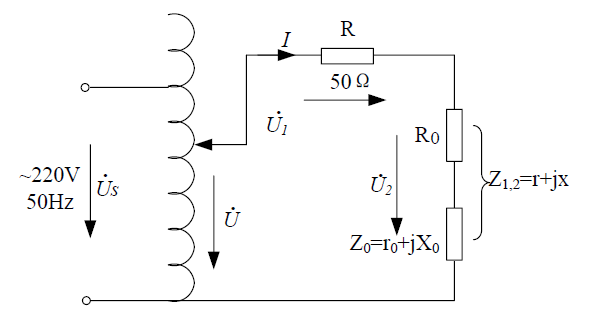
\includegraphics{pic/三电压表法电路图.png}
    \caption{三电压表法电路图}
    \label{fig:三电压表法电路图}
\end{figure}
接着,将这三个向量组成矢量图,如图\ref{fig:三电压表法矢量图}所示
\begin{figure}[!ht]
    \centering
    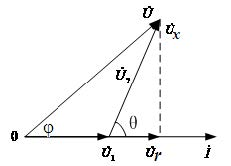
\includegraphics{pic/三电压表法矢量图.jpg}
    \caption{三电压表法矢量图}
    \label{fig:三电压表法矢量图}
\end{figure}
由余弦定理得
\begin{equation}
    \cos \theta = \dfrac{U^2-U_1^2-U_2^2}{2U_1U_2}
\end{equation}
再将$U_2$正交分解为电阻和电容(或电感)上的电压
\begin{equation}
    \begin{cases}
        U_r=U_2 \cos \theta\\
        U_x=U_2 \sin \theta
    \end{cases}
\end{equation}
于是我们得到关系
\begin{equation}
    \begin{cases}
        r=\dfrac{RU_r}{U_1}\\
        L=\dfrac{RU_x}{\omega U_1}\\
        C=\dfrac{U_1}{\omega R U_x}\\
        \cos \varphi = \dfrac{U_1+U_r}{U}=\dfrac{U_1+U_2\cos \theta}{U}
    \end{cases}
\end{equation}
这样,我们就得到了电阻、电感、电容、功率因数等单相交流电路参数的计算公式。
\subsubsection{三表法}
本实验使用三表合一的多功能测量平台。

搭建如图\ref{fig:三表法电路图}所示的电路
\begin{figure}[!ht]
    \centering
    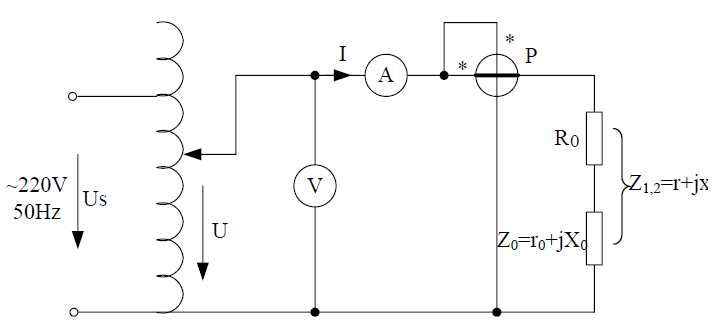
\includegraphics{pic/三表法电路图.png}
    \caption{三表法电路图}
    \label{fig:三表法电路图}
\end{figure}
以电源为基准相量,我们测量自耦变压器上的电压$\Dot{U}$,回路电流$\Dot{I}$以及未知阻抗上的功率$\Dot{P}$。由欧姆定律,满足
\begin{equation}
    z=\dfrac{U}{I}
\end{equation}
由有功功率的定义得到功率因数的表达式
\begin{equation}
    \cos \varphi =\dfrac{P}{UI}
\end{equation}
联立解得阻抗中的电阻部分
\begin{equation}
    r=\dfrac{P}{I^2}=z\cos \varphi
\end{equation}
解得电感或电容的阻抗
\begin{equation}
    X=\sqrt{z^2-r^2}=z\sin \varphi
\end{equation}
则电感或电容的参数为
\begin{equation}
    \begin{cases}
        L=\dfrac{X_L}{\omega}\\
        C=\dfrac{1}{X_C \omega}
    \end{cases}
\end{equation}
这样,我们就得到了电阻、电感、电容、功率因数等单相交流电路参数的计算公式。
\subsection{理论计算分析实验内容(3)中 Z1+Z2(Z1 串联 Z2)、,Z1//Z2(Z1 并联 Z2)时,电路的性质(容性电路还是感性电路)}
由题,$Z_1=R_1+L,Z_2=R_2+C,R_1=10\Omega,R_2=100\Omega,L=114mH,C=10\mu F$。$Z_1$与$Z_2$串联,电路总阻抗为
\begin{equation}
    Z=R_1+R_2+j\omega L+\dfrac{1}{j \omega C}=110-282.4957j(\Omega)
\end{equation}
电路总体呈现容性。

$Z_1$与$Z_2$并联,电路总阻抗为
\begin{equation}
    Z=\dfrac{(R_1+j\omega L)(R_2+\dfrac{1}{j\omega C})}{R_1+R_2+j(\omega L - \dfrac{1}{\omega C})}=13.6173+38.5922j(\Omega)
\end{equation}
电路总体呈现感性。
\subsection{复习功率因数概念,试列出负载功率因数改变(提高、减小)的方法}
功率因数是描述交流电路中有用功率和视在功率之间关系的参数。它表示电流相位相对于电压相位的偏移程度,即表征了负载对电网造成的功率损耗。功率因数的计算公式为:功率因数 = 有功功率 / 视在功率。其中,有功功率是负载实际消耗的功率,单位为瓦(W);视在功率是负载的功率总量,既包括有功功率,也包括无功功率,单位为伏安乘乘以安培(VA)。

改变功率因数的方法有:在电路中并联电容(推荐)或串联电容(不推荐);或者在电路中串联电感,或者在已有电感的基础上加装铁芯提高电感值。
\section{实验内容}
\subsection{三电压表法测量电路参数}
按照图\ref{fig:三电压表法电路图}连接电路。测得的数据为
\begin{table}[!ht]
    \centering
    \begin{tabular}{|c|c|c|c|c|c|c|c|c|c|}
    \hline
        ~ & $U(V)$ & $U_1(V)$ & $U_2(V)$ & $\cos \theta$ &$U_r(V)$ &$U_x(V)$ &$r_0(\Omega)$ &$L(mH)$ &$C(\mu)F$ \\ \hline
        $Z_1$ & 60&33.2&32.6&0.6629&21.6114&24.4071&32.5474&117.003&~\\ \hline
        $Z_2$&60&8.4&57.0&0.2929&16.6929&54.5009&99.3622& ~&9.8120\\ \hline
    \end{tabular}
    \caption{三电压表法测量电路参数}
    \label{tab:三电压表法测量电路参数}
\end{table}
可以看到,测量电感时,电阻值偏大。推测是因为电感线圈匝数较多,线阻较大。电感的测量误差为2.63\%,电容的测量误差为1.88\%,均在误差允许范围内。
\subsection{三表法测量电路参数}
按照图\ref{fig:三表法电路图}连接电路,测得电路参数为
\begin{table}[!ht]
    \centering
    \begin{tabular}{|c|c|c|c|c|c|c|c|c|c|}
    \hline
      ~& $I(A)$& $U(V)$ & $P(W)$ &$z(\Omega)$& $\cos \varphi$ & $r_0(\Omega)$&$x(\Omega)$&$L(mH)$ &$C(\mu)F$ \\ \hline    $Z_1$&0.3&14.6&3.20&48.6667&0.7306&35.5556&33.2302&105.775&~\\\hline   $Z_2$&0.3&98.9&9.06&329.667&0.3053&100.667&313.921&~&10.1398 \\    \hline$Z_1+Z_2$&0.3&94.3&12.34&314.333&0.4362&137.111&282.853&~&11.2535\\ \hline     $Z_1//Z_2$&0.3&15.7&3.90&52.333&0.8280&43.3333&29.3428&93.401&~\\ \hline
    \end{tabular}
    \caption{三表法测量电路参数}
    \label{tab:三表法测量电路参数}
\end{table}
\subsection{并联电容,改变功率因数}
仍按图\ref{fig:三表法电路图}接线,选取电容并联在负载 $Z_1$ 两端。首先调节单相自耦调压器,使副方电压
等于表 \ref{tab:三表法测量电路参数} 中负载为 $Z_1$ 时对应的电压值,然后测出 $I,P$,计算 $\cos \varphi$。
\begin{table}[!ht]
    \centering
    \begin{tabular}{|c|c|c|c|c|}
    \hline
        ~& $I(A)$ & $U(V)$ &$P(W)$ &$\cos\varphi$  \\ \hline
        原$Z_1$电路&0.3&14.6&3.20&0.7306\\ \hline 
        并联$8\mu F$电容 & 268.3m&14.4&3.07&0.7946\\\hline
        并联$16\mu F$电容 & 249.0m&14.4&3.08&0.8590\\\hline
    \end{tabular}
    \caption{并联电容,改变功率因数}
    \label{tab:并联电容,改变功率因数}
\end{table}
与不接电容前的负载功率因数相比较,发现并联电容后,电路中的电流减小,线上的电力损耗减少;与此同时,由于电路的电阻不变,所以有功功率不变,功率因数增大。
\subsection{电感插入铁芯,改变功率因数}
仍按图\ref{fig:三表法电路图}接线,将电感线圈中插入铁芯,调节调压器,观察电流表读数保持在 0.3A。
数据记录在表 \ref{tab:电感插入铁芯,改变功率因数}。
\begin{table}[!ht]
    \centering
    \begin{tabular}{|c|c|c|c|c|}
    \hline
        ~& $I(A)$ & $U(V)$ &$P(W)$ &$\cos\varphi$  \\ \hline
        原$Z_1$电路&0.3&14.6&3.20&0.7306\\ \hline 
        铁芯部分插入 & 0.3&19.9&3.35&0.5611\\\hline
    铁芯完全插入 & 0.3&60.3&3.37&0.1863\\\hline
    \end{tabular}
    \caption{电感插入铁芯,改变功率因数}
    \label{tab:电感插入铁芯,改变功率因数}
\end{table}
与未插入铁芯时数据比较,结合表格数据发现,插入铁芯后,副方线圈电压上升。但由于线圈的分压增大,所以电压增加的部分主要用在了无功功率上,有功功率变化不大,所以功率因数减小。
\subsection{改变电阻阻值,改变功率因数}
仍按图\ref{fig:三表法电路图}接线,改变$ Z_1$ 中串联的电阻阻值,调节调压器,观察电流表读数保持在 0.3A。采用串联电阻的方式增大回路电阻,增大后的电阻为20$\Omega$;采用并联电阻的方式减小电阻,减小后的电阻为$\dfrac{20}{3}=6.67\Omega$。完成表 5。
\begin{table}[!ht]
    \centering
    \begin{tabular}{|c|c|c|c|c|}
    \hline
        ~& $I(A)$ & $U(V)$ &$P(W)$ &$\cos\varphi$  \\ \hline
        原$Z_1$电路&0.3&14.6&3.20&0.7306\\ \hline 
        $Z_1$中电阻值增大 &0.3&16.8&4.03&0.7996\\\hline
     $Z_1$中电阻值减小 & 0.3&13.9&2.87&0。6882\\\hline
    \end{tabular}
    \caption{改变电阻阻值,改变功率因数}
    \label{tab:改变电阻阻值,改变功率因数}
\end{table}
增大电阻阻值,由于电流不变,所以电路的有功功率上升,无功功率不变,所以功率因数提高。若减小电阻阻值则反之。

\section{思考题}
\subsection{“并联电容”可以提高感性阻抗的功率因数,使用矢量图来分析并联的电容容量是否越大越好?}
一般情况下,当并联电容的值比较小时,整个电路的的电压矢量图如图\ref{fig:并联电容分析图1}所示
\begin{figure}[!ht]
    \centering
    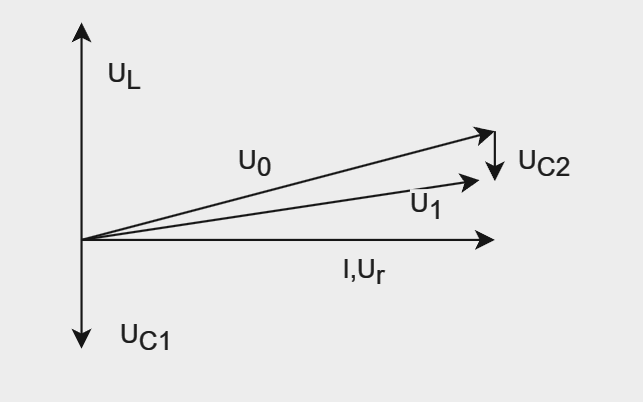
\includegraphics{pic/并联电容分析图1.png}
    \caption{并联电容分析图1}
    \label{fig:并联电容分析图1}
\end{figure}
在不并联电容时,电路的输入电压和回路电流夹角较大;并联电容后,$U_0$叠加一个向下的并联电容的分压$U_{C2}$,其叠加结果$U_1$与电流的夹角变小,功率因数提高。

但是,当并联电容的值不合适时,就会出现如图所示的情况。并联电容改变了电路的性质,从感性变成了容性,但是$U_1$与电流的夹角在另一侧仍然较大,功率因数不增反降。
\begin{figure}[!ht]
    \centering
    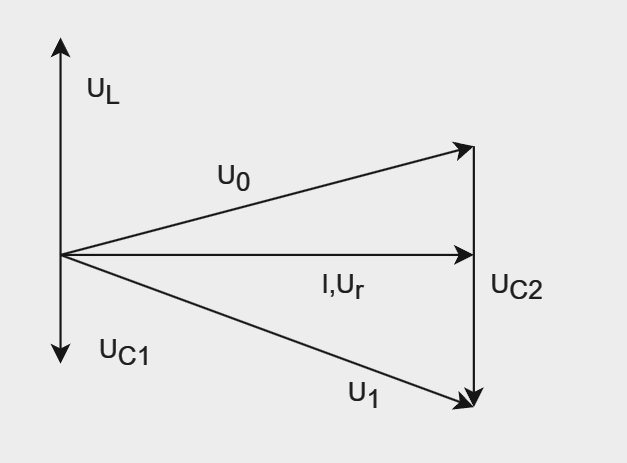
\includegraphics{pic/并联电容分析图2.png}
    \caption{并联电容分析图2}
    \label{fig:并联电容分析图2}
\end{figure}
\subsection{通过实验分析电感线圈中插入铁棒,电感值会有怎样变化?}
根据表四的数据可知,插入铁芯后,在电路电流没有改变的情况下,副方电压值上升而有功功率变化不大,说明无功功率增大,这意味着电感的电感值增大。
\subsection{使用矢量图分析 $Z_1$ 中串联的电阻阻值变化对功率因数的影响。}
分析电阻阻值增大的情况。如图\ref{fig:电阻分析图}所示,在电路电阻阻值较小的情况下,功率因数较大,增大电阻后,副方电压的垂直分量(电感部分)不变,水平分量增大(电阻部分分压提高),总电压与电流的夹角变小,功率因数提高。电阻阻值变小则相反。
\begin{figure}[!ht]
    \centering
    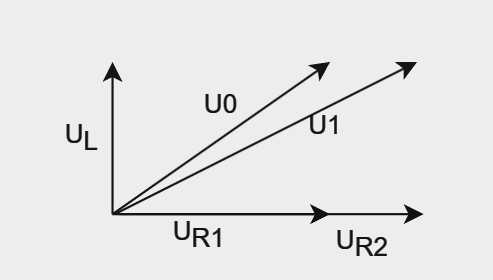
\includegraphics[scale=1.2]{pic/电阻分析图.png}
    \caption{电阻增大分析图}
    \label{fig:电阻分析图}
\end{figure}
\end{document}
